%!TEX root = ../thesis.tex
%*******************************************************************************
%****************************** Second Chapter *********************************
%*******************************************************************************

\chapter{Improving Cultural Competence in Computer Vision Machine Learning Algorithms}
\label{ch2v2}

\ifpdf
    \graphicspath{{Chapter2v2/Figs/Raster/}{Chapter2v2/Figs/PDF/}{Chapter2v2/Figs/}}
\else
    \graphicspath{{Chapter2v2/Figs/Vector/}{Chapter2v2/Figs/}}
\fi

%
This chapter introduces a specialized suite of task-specific Data Augmentation (DA) techniques designed to mitigate cultural bias within robotic visual perception frameworks. While the term data augmentation traditionally denotes a broad spectrum of domain-agnostic methodologies utilized to expand sample sizes, the strategies developed herein are intrinsically coupled with specific computer vision tasks. Due to its conceptual simplicity and empirical efficacy, data augmentation has been extensively explored within the vision domain. Crucially, although certain underlying principles introduced in this chapter can be generalized to alternative modalities, direct cross-domain transferability cannot be assumed a priori due to the distinct structural characteristics inherent to different data types.

\subsection{Oversampling Techniques}
\label{ch2:sec:os}
The most fundamental data augmentation (DA) strategy utilized is Oversampling (OS). 
In this approach, instances from under-represented cultural groups are replicated within the training distribution until an empirical balance across all cultural contexts is achieved.
A more sophisticated iteration of this technique, specifically designed for deep learning architectures, involves enforcing a Parity-Balanced Batch (PARB) strategy. 
Rather than static oversampling of the global dataset, PARB ensures that every stochastic gradient descent (SGD) iteration utilizes a mini-batch in which each cultural context $\mathcal{C}$ is represented with equal frequency.

\subsection{Random Transformations}
\label{ch2:sec:RT}
In various high-stakes applications~\citep{shorten2019survey}, particularly those involving high-dimensional input spaces such as computer vision, the empirical dataset $\mathcal{D}_n$ often lacks the cardinality required to fully encapsulate the underlying geometric and semantic invariances of the data-generating distribution $\mu$. 
To mitigate this limitation and suppress overfitting—thereby enhancing the generalization capabilities delineated in Section~\ref{ch2:sec:prel}—we utilize Random Transformations (RT).
Formally, we define a transformation mapping $T_\omega: \mathcal{X} \rightarrow \mathcal{X}$ parameterized by a random variable $\omega \in \Omega$. 
Here, $\Omega$ denotes the space of admissible transformations, which may include operations such as stochastic rotations, affine translations, or the injection of Gaussian noise. 
These transformations are constructed to be label-preserving, such that for any sample $(x_i, y_i) \in \mathcal{D}_n$, the augmented pair $(T_\omega(x_i), y_i)$ is assumed to represent a structurally valid realization from the support of $\mu$.

Within the scope of this research, we implement RT via two distinct operational strategies: Offline Random Transformation (OffRT) and Online Random Transformation (OnRT).
The OffRT approach involves the expansion of the training corpus $\mathcal{L}^r$ a priori, before the commencement of the training phase. 
We construct an augmented training set $\mathcal{L}^r_{\text{aug}} = \mathcal{L}^r \cup \{ (T_{\omega_i}(x_i), y_i) \}_{i=1}^{n_{\text{aug}}}$, where $n_{\text{aug}}$ denotes the cardinality of the synthesized samples. 
This effectively increases the sample size $n$ in Eq.~\eqref{ch2:eq:generalproblem}, facilitating the acquisition of a denser and more comprehensive representation of the input manifold.
Conversely, the OnRT strategy integrates the transformations dynamically into the model’s pipeline during the training phase. 
In this configuration, for every training epoch and each input instance $x$, a unique realization of $\omega$ is sampled, and the model processes the stochastically transformed input $T_\omega(x)$. 
This mechanism functions as a form of stochastic regularization—analogous to the dropout technique—thereby preventing the learning algorithm $\mathscr{A}_\mathcal{H}$ from memorizing specific training exemplars and instead incentivizing the extraction of invariant features.

Specifically, for the empirical evaluations conducted in this research, the space of admissible transformations $\Omega$ comprises horizontal reflections, stochastic rotations (within a bounded range of $g$ radians), the injection of additive Gaussian noise (with a standard deviation $\sigma = g$), and random rescaling (zooming). 
Within this framework, the variable $g$ serves as a scalar parameter governing the augmentation intensity of the RT methodology.

\subsection{Adversarial Sampling}
\label{ch2:sec:adv_sampling}

To further bolster the cultural competency of the classification framework, we incorporate an Adversarial Sampling (ADV) strategy. 
The fundamental intuition underlying this approach is to augment the training distribution with synthesized samples designed to compel the model to decouple cultural identifiers from the primary discriminative task.

This objective is operationalized through a specialized pre-training phase utilizing the Projected Gradient Descent (PGD) algorithm \citep{madry2017towards}. 
Within this paradigm, adversarial perturbations are iteratively generated to maximize the model's loss, effectively identifying the "weakest" points in the decision boundary across different cultural strata. By training on these challenging variants, the model is incentivized to ignore superficial cultural correlations and instead converge upon more robust, invariant features.

Initially, we train a cultural discriminator $D_{\Theta_D}: \mathcal{X} \rightarrow \mathbb{R}^{|\mathcal{C}|}$ designed to predict the cultural provenance of a given input. 
We implement two distinct variants of this architectural strategy: the instantiation of a single, monolithic global discriminator (NODIV) or, alternatively, the deployment of class-conditional discriminators (DIV).The discriminator's parameters are optimized by minimizing the categorical cross-entropy loss function:\begin{align}\mathcal{L}D(x, y{c}) = - \sum_{i=1}^{|\mathcal{C}|} y_{c,i} \log(D_{\Theta_D}(x)i),
\end{align}
where $y{c}$ represents the ground-truth cultural label.

Upon completion of the training phase for $D_{\Theta_D}$, we synthesize adversarial perturbations $\delta$ to construct augmented inputs $\tilde{x} = x + \delta$. 
This process utilizes the PGD framework, which iteratively updates the perturbation to maximize the cultural classification loss while constraining the transformation within a predefined $\epsilon$-ball of the original image. For an iteration $t$, the update rule is defined as follows:
%
\begin{align}
x_{t+1} = \Pi_{x+\mathcal{S}} \left( x_t + \alpha \cdot \text{sign} \left( \nabla_{x_t} \mathcal{L}D(D{\Theta_D}(x_t), y_{c}) \right) \right),
\end{align}
%
where $\alpha$ denotes the step size and $\Pi_{x+\mathcal{S}}$ represents the projection operator onto the feasible set $\mathcal{S}$. 
This set is governed by the $L_\infty$ norm constraint $\| \tilde{x} - x \|_\infty \leq \epsilon$ and the requisite pixel intensity bounds $[0, 1]$.

The final classification hypothesis $f_{\Theta}$ is optimized over an augmented dataset $\tilde{\mathcal{D}} = \mathcal{D}_n \cup \mathcal{D}_{adv}$, where the adversarial subset $\mathcal{D}_{adv}$ comprises the synthesized inputs $\tilde{x}$ paired with their corresponding ground-truth labels $y$. 
By training on instances where cultural markers have been stochastically shifted or obscured through adversarial perturbations, the model is incentivized to ignore culturally dependent artifacts. Consequently, the learning algorithm converges upon more robust, invariant features necessary for the primary discriminative task, thereby mitigating cultural bias and enhancing cross-cultural generalization.

\subsection{Diffusion Models}
\label{ch2:sec:diff_model}
The tertiary data augmentation (DA) strategy involves enriching the training corpus with synthetic imagery synthesized via a Diffusion Model (DM).Within the paradigm of generative modeling, the objective transitions from learning a discriminative mapping $f_\Theta: \mathcal{X} \rightarrow \mathcal{Y}$ to approximating the high-dimensional probability density function $\mu$ characterizing the input space $\mathcal{X}$. 
Diffusion models operationalize this by learning to invert a forward stochastic process that incrementally degrades the data through the sequential addition of Gaussian noise.

Consistent with the implementation provided in the framework, we define a diffusion schedule governed by a continuous temporal variable $t \in [0, 1]$. 
The transition from a noise-free image $x_0$ to its perturbed realization $x_t$ is characterized by the following linear interpolation:
%
\begin{equation}
x_t = \cos(\phi_t) x_0 + \sin(\phi_t) \epsilon, \quad \epsilon \sim \mathcal{N}(\mathbf{0}, \mathbf{I}),
\end{equation}
%
where the angular parameter $\phi_t$ is determined by a schedule that interpolates between a maximum signal-to-noise ratio (SNR) at $\cos(\phi_{\min}) = 0.95$ and a minimum SNR at $\cos(\phi_{\max}) = 0.02$. 
This specific trigonometric formulation ensures that the marginal variance of the latent variable $x_t$ remains invariant throughout the diffusion process, satisfying the constraint $\cos^2(\phi_t) + \sin^2(\phi_t) = 1$.

The model $f_\Theta$ is optimized to function as a denoiser. 
Specifically, the network architecture processes the perturbed image $x_t$ alongside the noise variance $\sin^2(\phi_t)$—which serves as a temporal conditioning signal—to predict the original noise component $\epsilon$. 
Consistent with the empirical risk minimization framework established in Problem~\eqref{ch2:eq:generalproblem}, the training objective employs the Mean Absolute Error (MAE) as the loss function $\ell$:
%
\begin{equation}
\min_\Theta \quad \hat{\mathbb{E}}_{\mathcal{D}n, \epsilon, t} \left| \epsilon - f\Theta(x_t, \sin^2\phi_t) \right|_1.
\end{equation}
%

To address our specific objective, the diffusion methodology may be operationalized by leveraging the complete training distribution $\mathcal{L}$ for a given class, or by restricting the generative process exclusively to instances associated with a minority cultural context (DMMIN).\begin{figure}\centering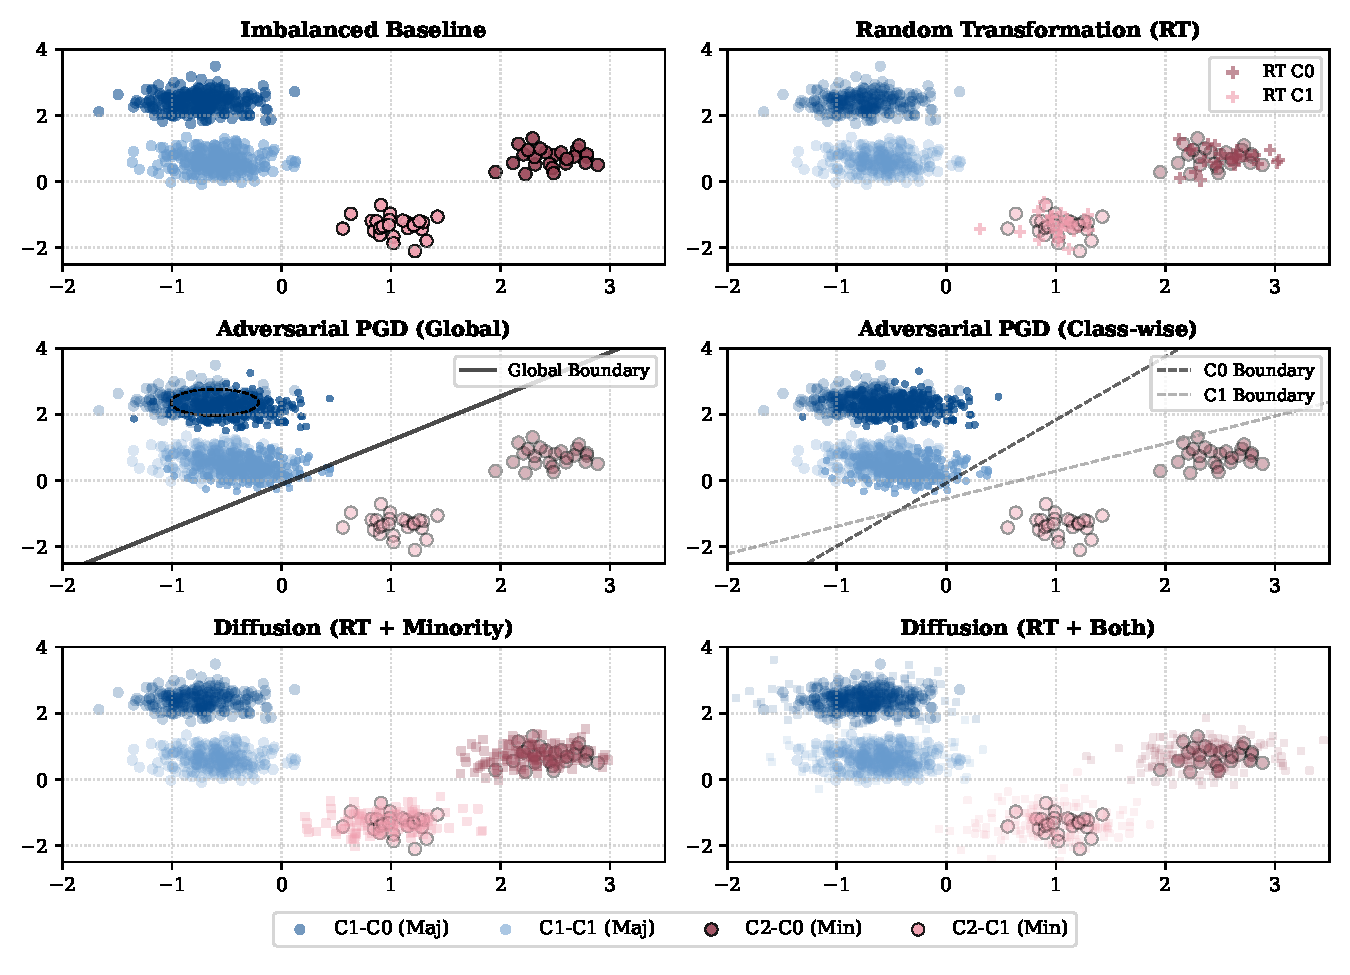
\includegraphics[width=1.0\linewidth]{Chapter2/Figs/mock_strategies_comparison.pdf}\caption{Simplified 2D feature-space visualizations illustrating the primary mitigation strategies delineated in this thesis.}\label{ch2:fig:mock_strategies_comparison}\end{figure}

\section{Combining MTL and DA}
\label{ch2:sec:mtl_and_da}
The mitigation strategies delineated above may be synergistically integrated to address specific operational requirements. 
Within the scope of this thesis, and primarily due to the inherent sparsity of the empirical dataset, diffusion-based augmentation methodologies are consistently coupled with RT. 
Specifically, the training corpus is first expanded via OffRT; this augmented distribution subsequently serves as the input for the diffusion process, further amplifying the dimensionality and density of the dataset.
Provided that the transformation $T_\omega$ remains invariant with respect to cultural identifiers, the integration of RT and MTL is a mathematically straightforward procedure. 
Conversely, the concatenation of synthetic instances generated via DM or DMMIN within an MTL framework presents greater complexity, as it requires the assignment of cultural labels to synthesized data. 
In this research, we adopt a heuristic wherein synthesized samples are stochastically assigned to a minority cultural context.

Individual mitigation techniques may also be concatenated sequentially to amplify the overall debiasing effect. 
Figure~\ref{ch2:fig:pipeline} illustrates the comprehensive integration of the proposed preprocessing strategies into a unified pipeline.

\begin{figure}
\centering
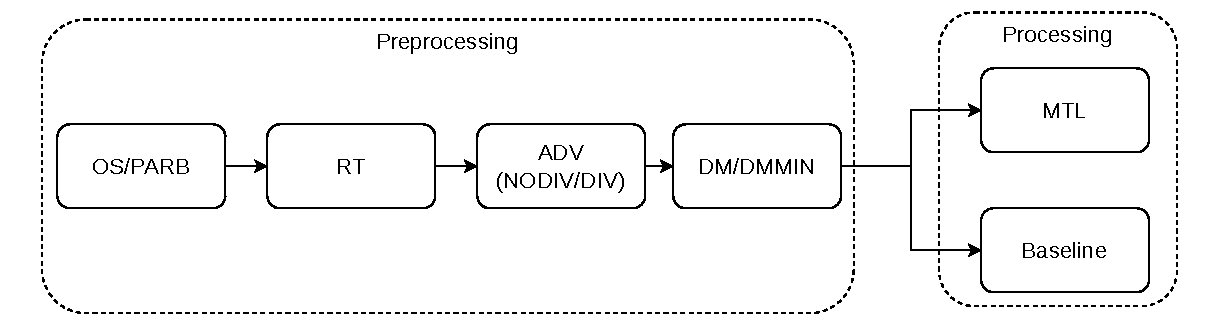
\includegraphics[width=1.0\linewidth]{Chapter2/Figs/DataAugmentationPipeline.drawio.pdf}
\caption{Schematic representation of the preprocessing and processing modules designed for the mitigation of cultural incompetence.}
\label{ch2:fig:pipeline}
\end{figure}

The presence of a diagonal slash within certain modules highlights a mutual exclusivity, necessitating a selection between alternative methodologies, such as OS and PARB. 
In principle, each data augmentation (DA) stratum can be stacked, whereby samples generated at one stage serve as the foundational input for the subsequent layer. 
Within this thesis, a exhaustive evaluation of every permutation of these DA techniques is not presented; instead, the specific combinations selected for empirical analysis are delineated in Chapter~\ref{ch3}.




